% Options for packages loaded elsewhere
\PassOptionsToPackage{unicode}{hyperref}
\PassOptionsToPackage{hyphens}{url}
\PassOptionsToPackage{dvipsnames,svgnames,x11names}{xcolor}
\documentclass[
  10pt,
  fontset=fandol]{ctexart}
\usepackage{xcolor}
\usepackage[margin=16mm]{geometry}
\usepackage{amsmath,amssymb}
\setcounter{secnumdepth}{-\maxdimen} % remove section numbering
\usepackage{iftex}
\ifPDFTeX
  \usepackage[T1]{fontenc}
  \usepackage[utf8]{inputenc}
  \usepackage{textcomp} % provide euro and other symbols
\else % if luatex or xetex
  \usepackage{unicode-math} % this also loads fontspec
  \defaultfontfeatures{Scale=MatchLowercase}
  \defaultfontfeatures[\rmfamily]{Ligatures=TeX,Scale=1}
\fi
\usepackage{lmodern}
\ifPDFTeX\else
  % xetex/luatex font selection
\fi
% Use upquote if available, for straight quotes in verbatim environments
\IfFileExists{upquote.sty}{\usepackage{upquote}}{}
\IfFileExists{microtype.sty}{% use microtype if available
  \usepackage[]{microtype}
  \UseMicrotypeSet[protrusion]{basicmath} % disable protrusion for tt fonts
}{}
\makeatletter
\@ifundefined{KOMAClassName}{% if non-KOMA class
  \IfFileExists{parskip.sty}{%
    \usepackage{parskip}
  }{% else
    \setlength{\parindent}{0pt}
    \setlength{\parskip}{6pt plus 2pt minus 1pt}}
}{% if KOMA class
  \KOMAoptions{parskip=half}}
\makeatother
\usepackage{longtable,booktabs,array}
\newcounter{none} % for unnumbered tables
\usepackage{calc} % for calculating minipage widths
% Correct order of tables after \paragraph or \subparagraph
\usepackage{etoolbox}
\makeatletter
\patchcmd\longtable{\par}{\if@noskipsec\mbox{}\fi\par}{}{}
\makeatother
% Allow footnotes in longtable head/foot
\IfFileExists{footnotehyper.sty}{\usepackage{footnotehyper}}{\usepackage{footnote}}
\makesavenoteenv{longtable}
\usepackage{graphicx}
\makeatletter
\newsavebox\pandoc@box
\newcommand*\pandocbounded[1]{% scales image to fit in text height/width
  \sbox\pandoc@box{#1}%
  \Gscale@div\@tempa{\textheight}{\dimexpr\ht\pandoc@box+\dp\pandoc@box\relax}%
  \Gscale@div\@tempb{\linewidth}{\wd\pandoc@box}%
  \ifdim\@tempb\p@<\@tempa\p@\let\@tempa\@tempb\fi% select the smaller of both
  \ifdim\@tempa\p@<\p@\scalebox{\@tempa}{\usebox\pandoc@box}%
  \else\usebox{\pandoc@box}%
  \fi%
}
% Set default figure placement to htbp
\def\fps@figure{htbp}
\makeatother
\setlength{\emergencystretch}{3em} % prevent overfull lines
\providecommand{\tightlist}{%
  \setlength{\itemsep}{0pt}\setlength{\parskip}{0pt}}
\usepackage{amsmath,amssymb,mathtools,needspace}
\xeCJKDeclareCharClass{CJK}{"2032,"0400->"04FF,"2160->"216B,"2460->"2473,"25A0,"25C7,"25CB,"25CF}
\IfFontExistsTF{Arial Unicode MS}{\xeCJKsetup{AutoFallBack=true}\setCJKfallbackfamilyfont{\CJKrmdefault}{Arial Unicode MS}}{}
\setcounter{secnumdepth}{0}
\setlength{\emergencystretch}{2em}
\allowdisplaybreaks
\usepackage{bookmark}
\IfFileExists{xurl.sty}{\usepackage{xurl}}{} % add URL line breaks if available
\urlstyle{same}
\hypersetup{
  pdftitle={差商及其性质},
  colorlinks=true,
  linkcolor={Maroon},
  filecolor={Maroon},
  citecolor={Blue},
  urlcolor={Blue},
  pdfcreator={LaTeX via pandoc}}

\title{差商及其性质}
\author{}
\date{}

\begin{document}
\maketitle

\subsubsection{2.4.1 差商及其性质}\label{ux5deeux5546ux53caux5176ux6027ux8d28}

Lagrange 插值公式可以看作直线方程两点式的推广，如果从点斜式直线方程

\[
P_1(x)=f_0+\frac{f_1-f_0}{x_1-x_0}(x-x_0)
\]

出发，将它推广到具有 \(n+1\) 个插值点 \((x_0,\allowbreak f_0),\allowbreak (x_1,\allowbreak f_1),\allowbreak \cdots,\allowbreak (x_n,\allowbreak f_n)\) 的情况，则可把插值多项式表示为

\[
\begin{aligned}
P_n(x)={}&a_0+a_1(x-x_0)+a_2(x-x_0)(x-x_1)+\cdots\\
&+a_n(x-x_0)\cdots(x-x_{n-1}),
\end{aligned}
\tag{2.4.1}
\]

其中 \(a_0,a_1,\cdots,a_n\) 为待定系数，可由插值条件 \(P_n(x_j)=f_j\;(j=0,1,\cdots,n)\) 确定。

当 \(x=x_0\) 时，\(P_n(x_0)=a_0=f_0\)；当 \(x=x_1\) 时，\(P_n(x_1)=a_0+a_1(x-x_0)=f_1\)，推得

\[
a_1=\frac{f_1-f_0}{x_1-x_0};
\]

当 \(x=x_2\) 时，\(P_n(x_2)=a_0+a_1(x_2-x_0)+a_2(x_2-x_0)(x_2-x_1)=f_2\)，

推得

\[
a_2=\frac{\dfrac{f_2-f_0}{x_2-x_0}-\dfrac{f_1-f_0}{x_1-x_0}}{x_2-x_1}.
\]

依此递推，可得到 \(a_3,a_4,\cdots,a_n\)。为写出系数 \(a_k\) 的一般表达式，先引进如下差商定义。

\textbf{定义 2.3} 称 \(f[x_0,x_k]=\dfrac{f(x_k)-f(x_0)}{x_k-x_0}\) 为函数 \(f(x)\) 关于点 \(x_0,x_k\) 的一阶差商，称

\begin{quote}
定义 2.3 续 PDF 37。
\end{quote}

\subsubsection{校注（agent 补充）：代入行的原书记号}\label{ux6821ux6ce8agent-ux8865ux5145ux4ee3ux5165ux884cux7684ux539fux4e66ux8bb0ux53f7}

上面``当 \(x=x_1\) 时''一行，扫描原书实际写成 \(a_0+a_1(x-x_0)\)，其中 \(x\) 没有下标 \(1\)，本转录予以保留。在该行已经限定的 \(x=x_1\) 条件下，求系数时即代入 \(x_1\)；不将这一记号静默改写成原文没有印出的 \(a_1(x_1-x_0)\)。原页的 \(a_2\) 分式有整体分母 \(x_2-x_1\)，OCR 漏掉了这一层分母，本转录已恢复。

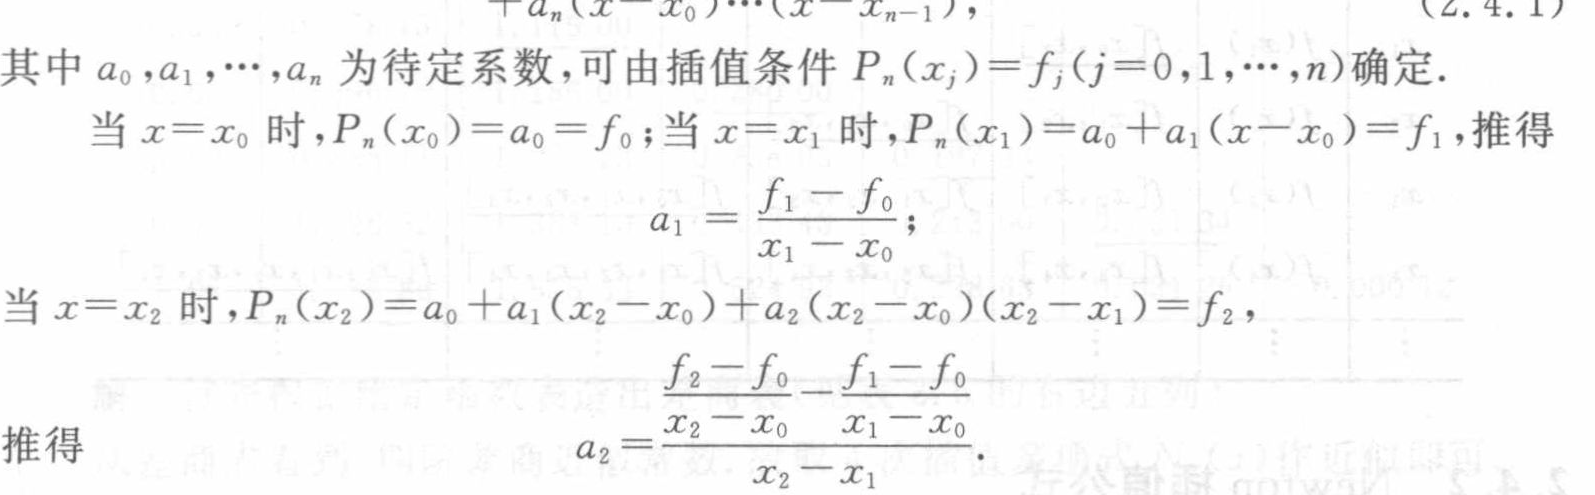
\includegraphics[width=0.85\linewidth,height=\textheight,keepaspectratio,alt={PDF 36 代入与系数原图裁切}]{../assets/ch02a/pdf-036-coefficients-detail.png}

\href{../../source-images/pdf-037.jpeg}{原页：书页 24／PDF 37}

\begin{quote}
页首承接 PDF 36 的定义 2.3；页末递推式续 PDF 38。
\end{quote}

\[
f[x_0,x_1,x_k]=\frac{f[x_0,x_k]-f[x_0,x_1]}{x_k-x_1}
\]

为 \(f(x)\) 关于点 \(x_0,x_1,x_k\) 的二阶差商。一般地，称

\[
f[x_0,x_1,\cdots,x_k]=\frac{f[x_0,x_1,\cdots,x_{k-2},x_k]-f[x_0,x_1,\cdots,x_{k-1}]}{x_k-x_{k-1}}
\tag{2.4.2}
\]

为 \(f(x)\) 的 \(k\) 阶差商。

差商有如下的基本性质：

（1）\(k\) 阶差商可表示为函数值 \(f(x_0),f(x_1),\cdots,f(x_k)\) 的线性组合，即

\[
f[x_0,x_1,\cdots,x_k]=\sum_{j=0}^{k}\frac{f(x_j)}{(x_j-x_0)\cdots(x_j-x_{j-1})(x_j-x_{j+1})\cdots(x_j-x_k)}.
\tag{2.4.3}
\]

这个性质可用归纳法证明。这个性质也表明差商与节点的排列次序无关，称为差商的对称性，即

\[
f[x_0,x_1,\cdots,x_k]=f[x_1,x_0,x_2,\cdots,x_k]=\cdots=f[x_1,x_2,\cdots,x_k,x_0].
\]

（2）由性质（1）及式（2.4.2）可得

\[
f[x_0,x_1,\cdots,x_k]=\frac{f[x_1,x_2,\cdots,x_k]-f[x_0,x_1,\cdots,x_{k-1}]}{x_k-x_0}.
\tag{2.4.4}
\]

（3）若 \(f(x)\) 在 \([a,b]\) 上存在 \(n\) 阶导数，且节点 \(x_0,x_1,\cdots,x_n\in[a,b]\)，则 \(n\) 阶差商与导数关系为

\[
f[x_0,x_1,\cdots,x_n]=\frac{f^{(n)}(\xi)}{n!},\qquad\xi\in[a,b].
\tag{2.4.5}
\]

这个公式可直接用 Rolle 定理证明。

差商的其他性质还可见本章习题。差商计算可列差商表如表 2.4 所示。

\textbf{表 2.4}

{\def\LTcaptype{none} % do not increment counter
\begin{longtable}[]{@{}
  >{\raggedright\arraybackslash}p{(\linewidth - 10\tabcolsep) * \real{0.1667}}
  >{\raggedright\arraybackslash}p{(\linewidth - 10\tabcolsep) * \real{0.1667}}
  >{\raggedright\arraybackslash}p{(\linewidth - 10\tabcolsep) * \real{0.1667}}
  >{\raggedright\arraybackslash}p{(\linewidth - 10\tabcolsep) * \real{0.1667}}
  >{\raggedright\arraybackslash}p{(\linewidth - 10\tabcolsep) * \real{0.1667}}
  >{\raggedright\arraybackslash}p{(\linewidth - 10\tabcolsep) * \real{0.1667}}@{}}
\toprule\noalign{}
\begin{minipage}[b]{\linewidth}\raggedright
\(x_k\)
\end{minipage} & \begin{minipage}[b]{\linewidth}\raggedright
\(f(x_k)\)
\end{minipage} & \begin{minipage}[b]{\linewidth}\raggedright
一阶差商
\end{minipage} & \begin{minipage}[b]{\linewidth}\raggedright
二阶差商
\end{minipage} & \begin{minipage}[b]{\linewidth}\raggedright
三阶差商
\end{minipage} & \begin{minipage}[b]{\linewidth}\raggedright
四阶差商
\end{minipage} \\
\midrule\noalign{}
\endhead
\bottomrule\noalign{}
\endlastfoot
\(x_0\) & \(\underline{f(x_0)}\) & & & & \\
\(x_1\) & \(f(x_1)\) & \(\underline{f[x_0,x_1]}\) & & & \\
\(x_2\) & \(f(x_2)\) & \(f[x_1,x_2]\) & \(\underline{f[x_0,x_1,x_2]}\) & & \\
\(x_3\) & \(f(x_3)\) & \(f[x_2,x_3]\) & \(f[x_1,x_2,x_3]\) & \(\underline{f[x_0,x_1,x_2,x_3]}\) & \\
\(x_4\) & \(f(x_4)\) & \(f[x_3,x_4]\) & \(f[x_2,x_3,x_4]\) & \(f[x_1,x_2,x_3,x_4]\) & \(\underline{f[x_0,x_1,x_2,x_3,x_4]}\) \\
\(\vdots\) & \(\vdots\) & \(\vdots\) & \(\vdots\) & \(\vdots\) & \(\vdots\) \\
\end{longtable}
}

\end{document}
